This chapter gives a brief overview of what messaging is and how it can be used for system integration purposes. It introduces various messaging patterns which will be used by the technological integration in chapter 4 and 5.
The content of this chapter is based on the book \textit{Enterprise Integration Patterns} by \textcite{EIP}.

Messaging is an asynchronous system-to-system communication, delivering packages of data called messages through channels. Messages can contain any structured data like strings, arrays or objects. It is up to the sender and receiver to determine and understand its content.

Channels can be seen as a queue of messages, accessible to interested systems. Channels have a direction in a sense so that no system simultaneously writes to and reads from a channel. Therefore, by one system writing messages to a channel and another system reading them, a message and data flow can be established.

Depending on the use case, the flow and destination of messages might have to be determined during operation. Therefore, various message routing components exist. Their purpose is to transfer messages from an inbound channel to one or more outbound channels, depending on predefined or dynamic rules.

During the routing of messages between systems, the content of messages might have to be modified. Therefore various message transformation components exist. Their purpose is to consume messages from an inbound channel, modify their content based on predefined or dynamic rules and publish the modified message to an outbound channel.

"\textit{A messaging system manages messaging the way a database system manages data persistence}" \cite[p. 31]{EIP}. Configuring a messaging system involves definition of available channels, the type of messages they exchange, their connection between systems, the message flow and when necessary the insertion of routing and transformation components.

Depending on the messaging system solution, additional features can be configured to increase performance, stability, failure safety and more. If properly configured, the messaging system operates reliably, handles unreliable network connections and persistently stores messages in case of a system crash.

\subsection{Messaging Integration}

One use case for a messaging system is integration.

The main benefit of messaging for integration is that it enables systems to share services and data in a decoupled way. Neither system, whether sending or receiving messages, needs to be aware of each other. 

During configuration of the messaging system, datatype channels can be defined. On these channels, only messages with the same content are exchanged. Using message transformation components, messages placed on a datatype channel can be translated to follow a canonical data model.

Systems consuming messages from datatype channels can individually assign a purpose to channels independent from the sending system. As a result of the canonical data model, receiving systems can also choose a data structure independent from the sending system.

As channels are able to function as a message buffer, sender and receiver of messages do not even have to be running at the same time.

\subsection{Messaging Patterns}

In the book "\textit{Enterprise Integration Patterns}" by \cite{EIP} multiple patterns for designing messaging systems are presented. This section gives a brief overview of patterns relevant for the thesis and their visual notation. Lucidchart \cite{lucid} was used for drawing messaging figures.

\paragraph{Message}

Figure \ref{messaging:message} shows the visual notation of a message with two attributes. 

\begin{figure}[H]
    \centering
    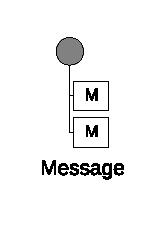
\includegraphics[scale=0.6]{Diagrams/Messaging/1. Message.pdf}
    \caption{Message}
    \label{messaging:message}
\end{figure}

\paragraph{Channel}

Figure \ref{messaging:channel1} shows the visual notation of an unnamed channel. Arrows to a message symbol are not a notation for channels but for message flow.

\begin{figure}[H]
    \centering
    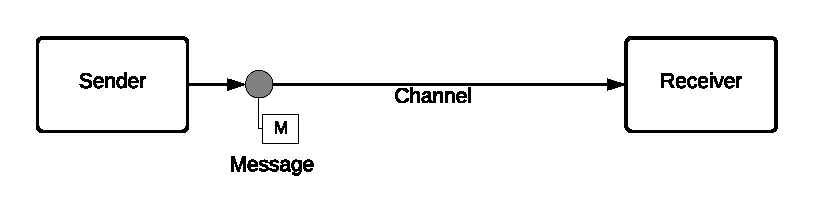
\includegraphics[scale=0.6]{Diagrams/Messaging/3. Channel.pdf}
    \caption{Unnamed Channel}
    \label{messaging:channel1}
\end{figure}

Figure \ref{messaging:channel2} shows the visual notation of a named channel. Arrows to and from named channels are not a notation for channels but for message flow. Channels are named if they have special importance.

There are different types of channels. In this thesis, named channels are publish-subscribe datatype channels. Unnamed channels are point-to-point channels. Publish-subscribe channels can be accessed by every system. In contrast to that, point-to-point channels can only be accessed by two systems - one writing and one reading system.

\begin{figure}[H]
    \centering
    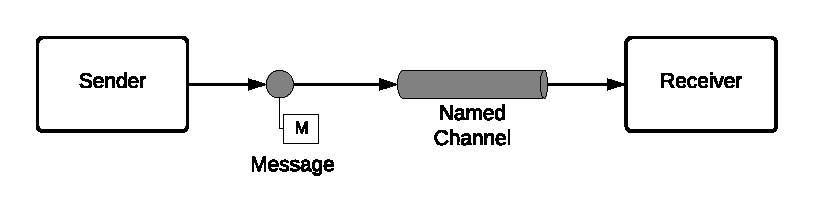
\includegraphics[scale=0.6]{Diagrams/Messaging/2. Channel.pdf}
    \caption{Named Channel}
    \label{messaging:channel2}
\end{figure}

\paragraph{Messaging Adapter}

Systems that do not natively support message based communication require a messaging adapter which enables the programs of the system to access the messaging system through an API. The messaging adapter usually has to be developed individually for each system, and manually integrated into the code of the system through asynchronous function calls of the adapter API.

Figure \ref{messaging:adapter} shows the visual notation of a Messaging Adapter connected to a system.

\begin{figure}[H]
    \centering
    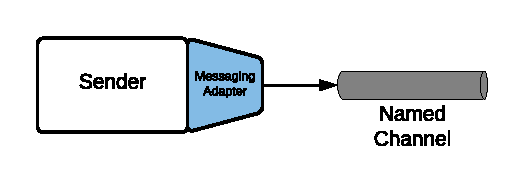
\includegraphics[scale=0.6]{Diagrams/Messaging/4. Messaging Adapter.pdf}
    \caption{Messaging Adapter}
    \label{messaging:adapter}
\end{figure}

\paragraph{Content-Based Router}

Content-Based Routers contain a preconfigured set of routing rules, that instruct the router to place inbound messages on different outbound channels depending on their content. These rules do not change during operation of the system.

Figure \ref{messaging:router} shows the visual notation of a Message Router.

\begin{figure}[H]
    \centering
    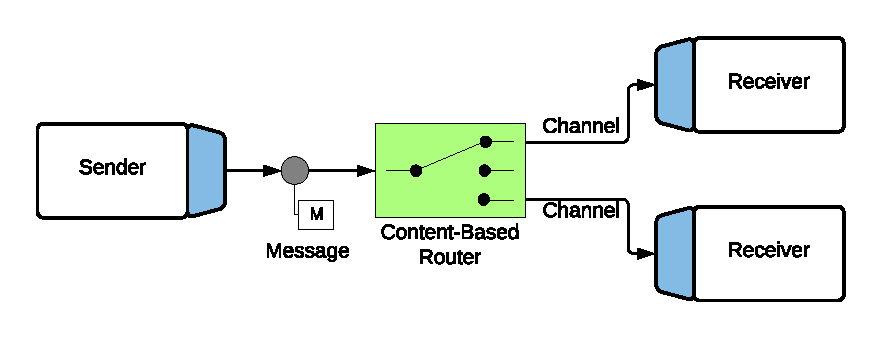
\includegraphics[scale=0.6]{Diagrams/Messaging/5. Message Router.pdf}
    \caption{Message Router}
    \label{messaging:router}
\end{figure}

\paragraph{Message Translator}

Message Translators have the purpose of translating message content on data representation and data type layer. 
On the data representation layer, message translators translate message content for example from an XML format to a JSON format. On the data type layer, message translators can for example concatenate first name and last name fields to a single name field.

Figure \ref{messaging:translator1} shows the visual notation of a Message Translator.

\begin{figure}[H]
    \centering
    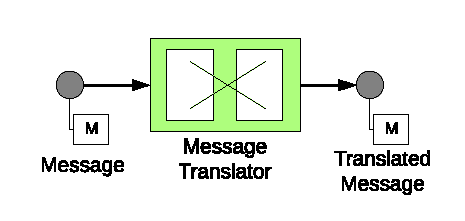
\includegraphics[scale=0.6]{Diagrams/Messaging/6. Message Translator.pdf}
    \caption{Message Translator}
    \label{messaging:translator1}
\end{figure}

As shown in figure \ref{messaging:translator2}, if using two message translators on both sides of a channel, a canonical data model can be created in between. For more information, read \textcite[p. 355]{EIP}.

\begin{figure}[H]
    \centering
    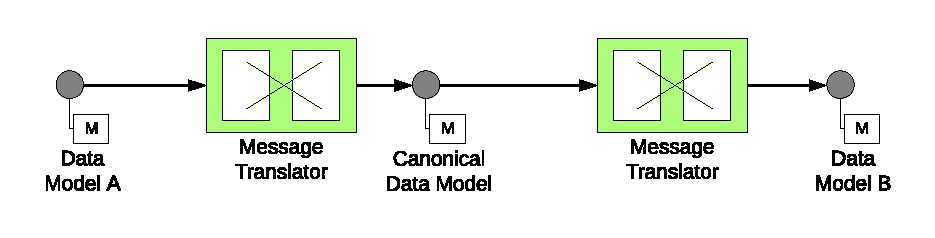
\includegraphics[scale=0.6]{Diagrams/Messaging/7. Message Translator.pdf}
    \caption{Message Translator creating Canonical Data Model}
    \label{messaging:translator2}
\end{figure}

\paragraph{Message Filter}

Message Filters contain a preconfigured set of filtering rules that instruct the filter to delete messages based on their content. These rules do not change during operation of the system.

Figure \ref{messaging:filter1} shows the visual notation of a Message Filter.

\begin{figure}[H]
    \centering
    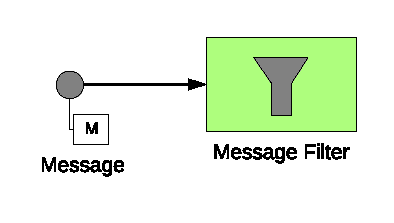
\includegraphics[scale=0.6]{Diagrams/Messaging/8. Message Filter.pdf}
    \caption{Message Filter}
    \label{messaging:filter1}
\end{figure}

As shown in figure \ref{messaging:filter2}, Message Filters can, in combination with publish-subscribe channels, be used to separate messages onto individual datatype channels.

\begin{figure}[H]
    \centering
    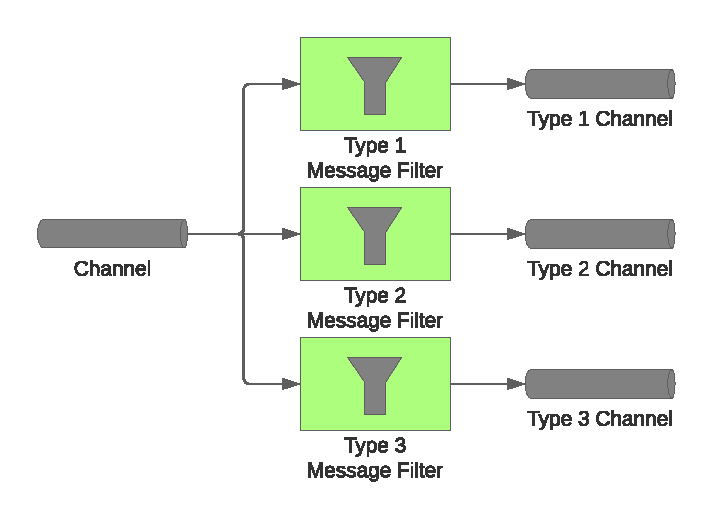
\includegraphics[scale=0.6]{Diagrams/Messaging/9. Message Filter.pdf}
    \caption{Message Filter separating Message Types}
    \label{messaging:filter2}
\end{figure}

\paragraph{Content Enricher}

Content Enricher have the purpose of adding new attributes to messages. The content which is usually added is a predetermined set of attributes but with dynamically created values.

Figure \ref{messaging:enricher} shows the visual notation of a Content Enricher.


\begin{figure}[H]
    \centering
    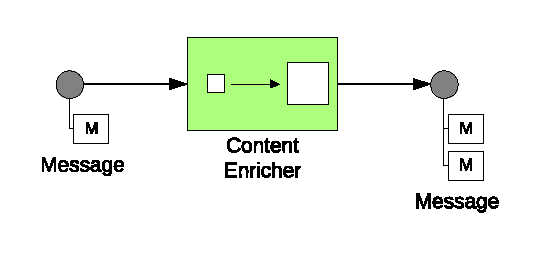
\includegraphics[scale=0.6]{Diagrams/Messaging/10. Content Enricher.pdf}
    \caption{Content Enricher}
    \label{messaging:enricher}
\end{figure}

\paragraph{Content Filter}

Content filters have the purpose of removing a predetermined set of attributes from messages.

Figure \ref{messaging:filter3} shows the visual notation of a Content Filter.

\begin{figure}[H]
    \centering
    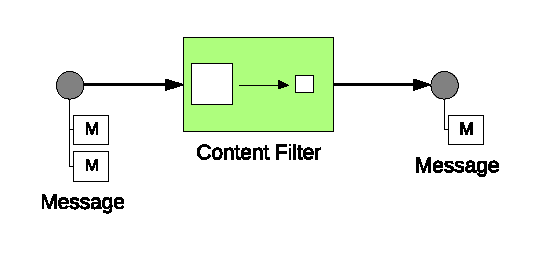
\includegraphics[scale=0.6]{Diagrams/Messaging/11. Content Filter.pdf}
    \caption{Content Filter}
    \label{messaging:filter3}
\end{figure}

\paragraph{Message Store}

Message Stores have the purpose of storing consumed messages in a database. They are also capable of communicating with other messaging patterns for providing access to stored messages. Communication between message patterns and Message Stores is indicated by a dotted arrow.

Figure \ref{messaging:store} shows the visual notation of a Message Store. It also shows the example of a Content Enricher accessing the message store.

\begin{figure}[H]
    \centering
    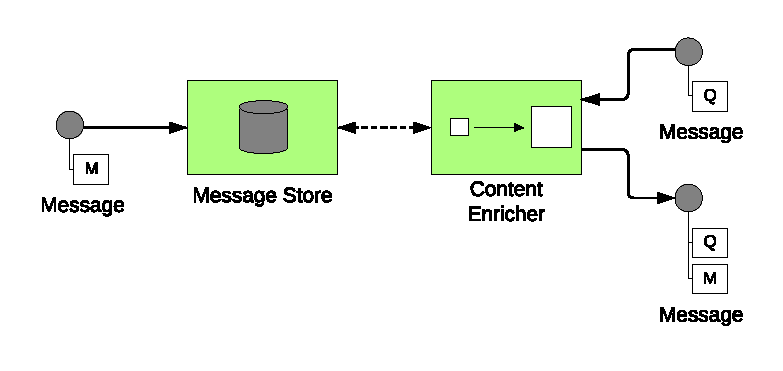
\includegraphics[scale=0.6]{Diagrams/Messaging/12. Message Store.pdf}
    \caption{Message Store}
    \label{messaging:store}
\end{figure}

